%BESCHREIBUNG DER FUNKTIONEN!
\subsection{Beschreibung der Funktionen}
Das Projekt besteht hauptsächlich aus drei Teilen.
Einer Website, auf welcher die Statusanzeigen der 
einzelnen Wallboxen und andere Funktionen angezeigt
werden, einen Charge Controller, welcher dafür 
verantwortlich ist, die Befehle der GUI entgegenzunehmen 
und auszuwerten, und aus einem Gateway, welches zwischen 
den Controllern und dem Modbus-Adapter liegt. Wenn also 
jemand eine Ladestation einschaltet, schickt die Website 
(HMI (Human Machine Interface)) über die Flexcloud einen 
Befehl zu dem Charge Controller. 
Siehe Aufbau des Projektes: \ref{fig:impl:Infografik_FlexBoxen}.

  \begin{figure}
    \centering
    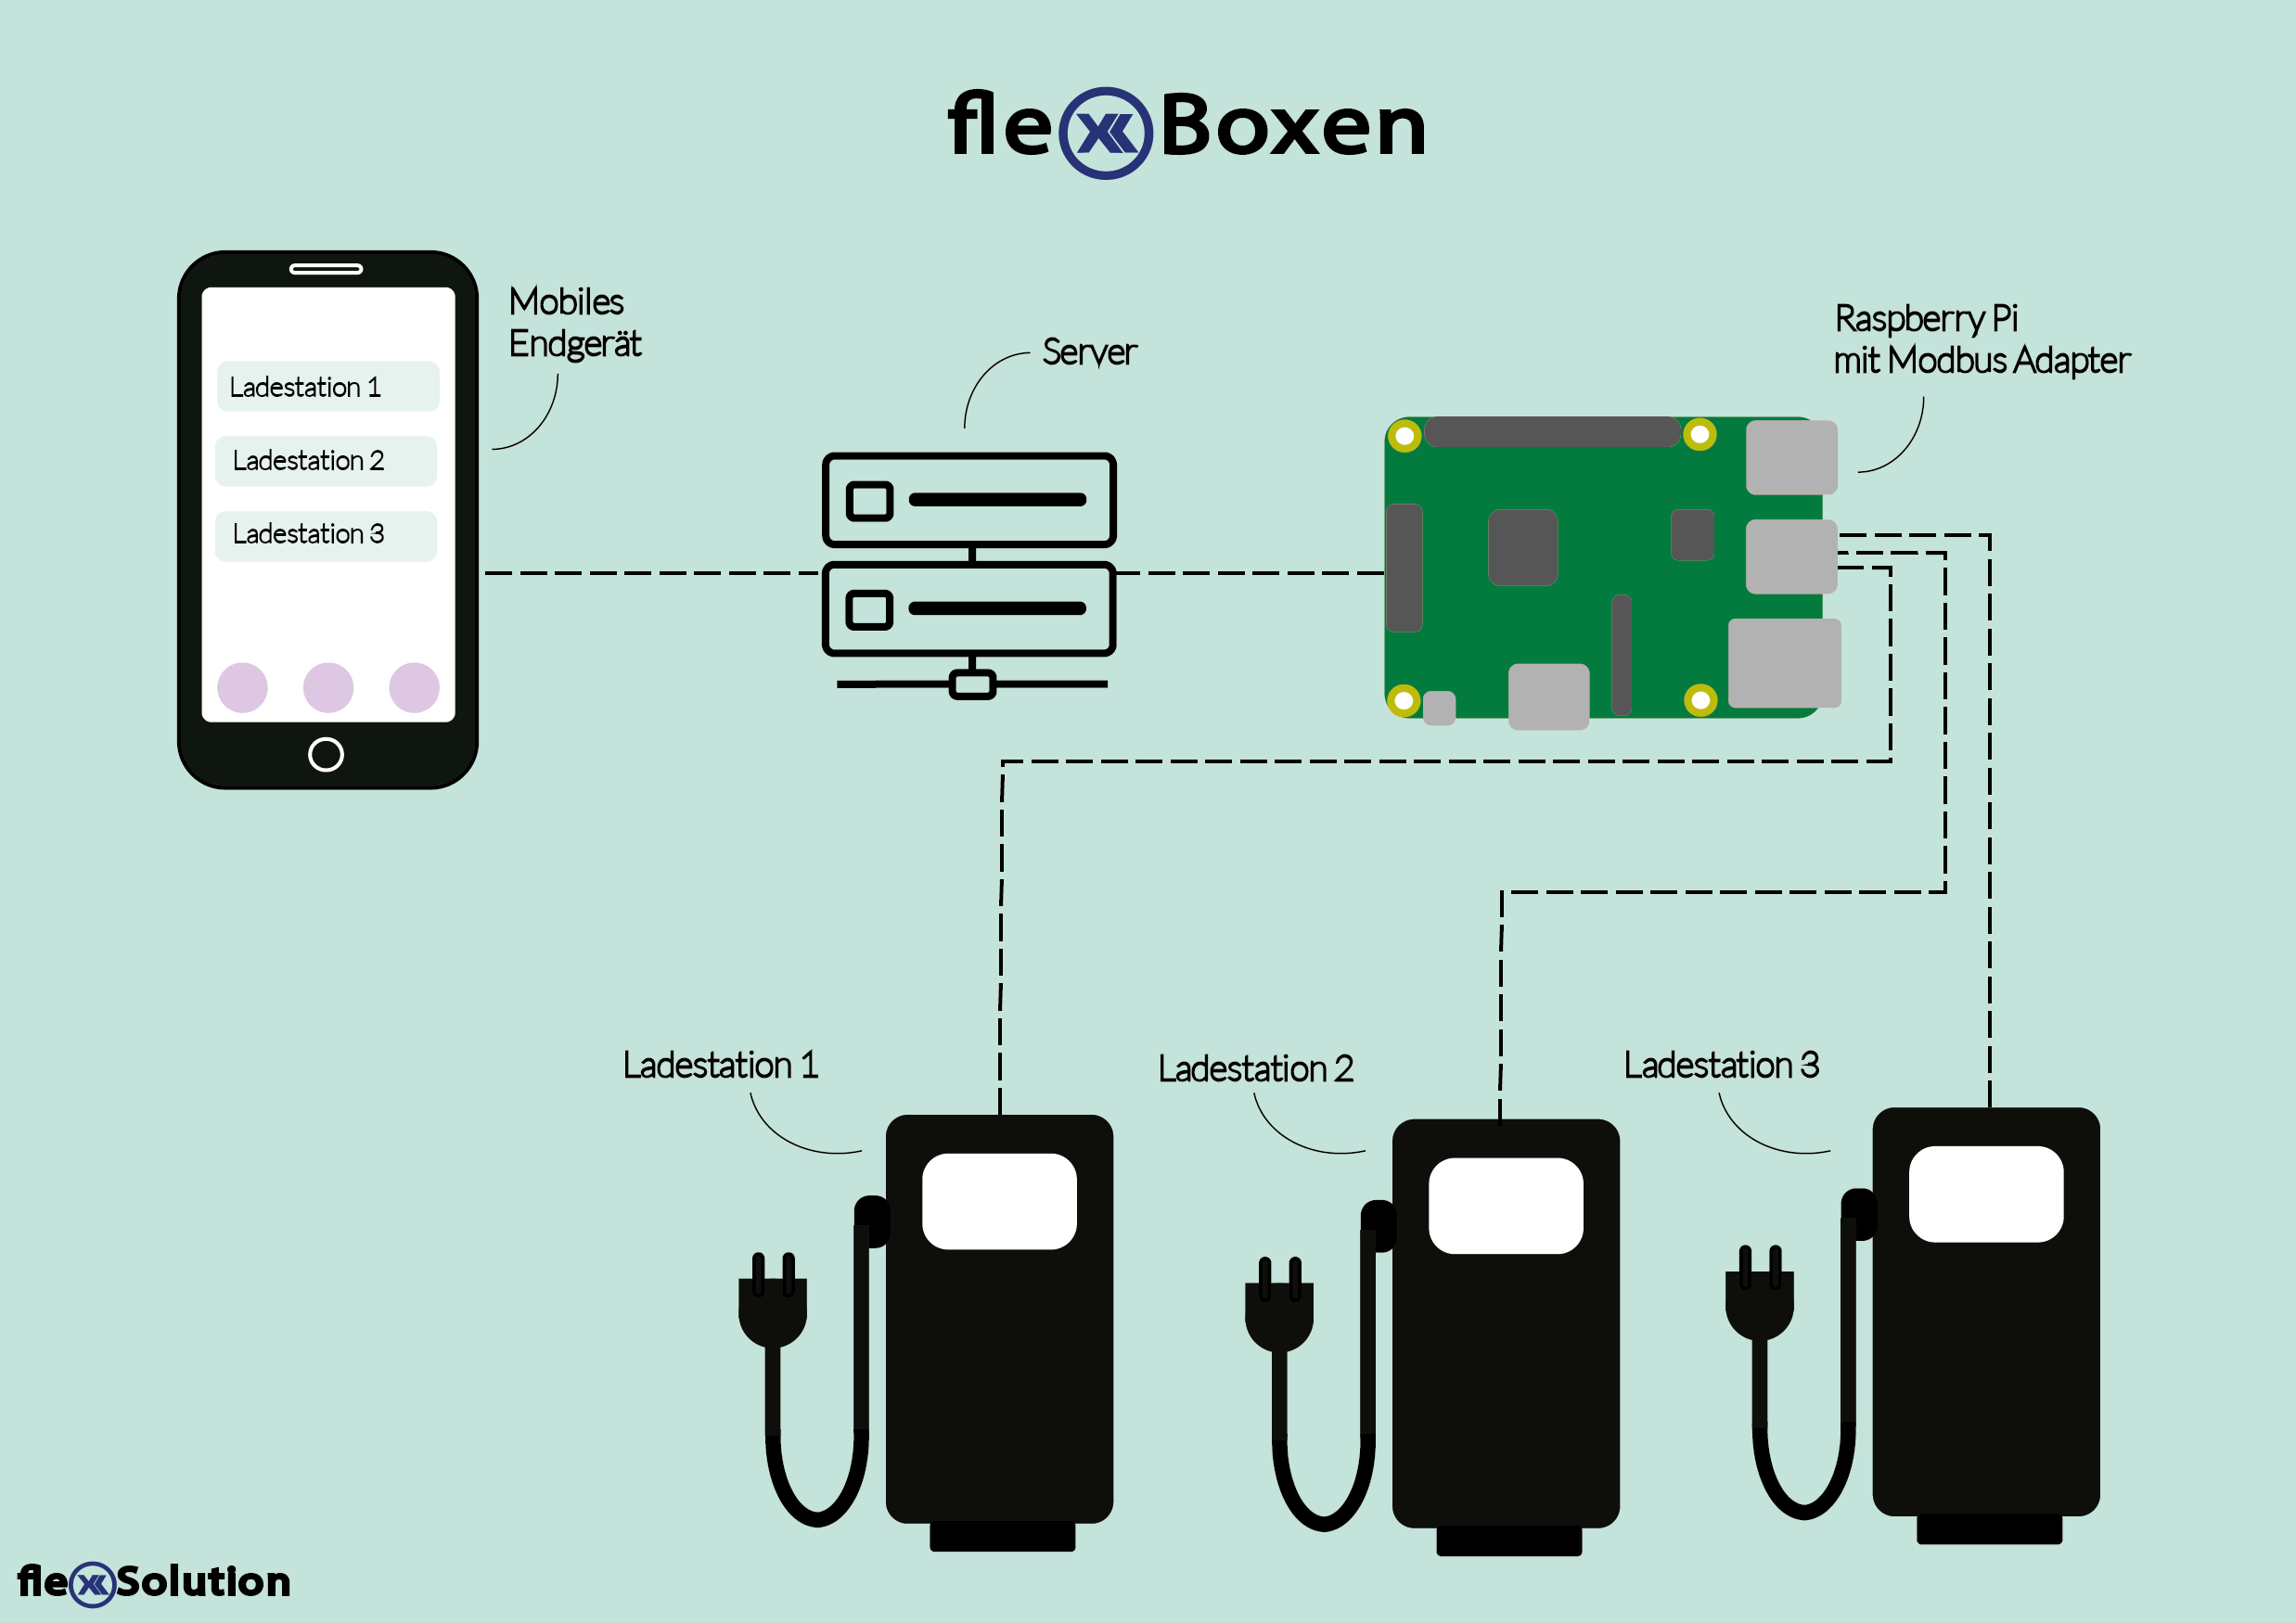
\includegraphics[scale=0.5]{pics/Infografik_FlexBoxen.png}
    \caption{Darstellung des Aufbaues}
    \label{fig:impl:Infografik_FlexBoxen}
\end{figure}




% WALLBOXEN

\subsection{Beschreibung der Wallboxen}

Die Wallboxen sind 5 Ladestationen der Marke "I-Charge". Sie wurden im August 2021 an einer Außenwand der Firma montiert. Jede einzelne ist mit 400 Volt an das Stromnetz der Firma gebunden, und kann mit bis zu 32 A bzw. 22 kWh Leistung das Auto laden. Um den Status der Wallbox überwachen zu können, gibt es an der Vorderseite des Panels eine LED-Anzeige mit 5 Punkten, welche in verschiedenen Farben leuchten können. 
grün durchgehend: Station ist frei 
blau blinkend: Station ist besetzt, das Auto lädt aber nicht, weil es entweder voll oder die Wallbox ausgeschalten ist 
blau durchgehend: Station ist besetzt, das Auto lädt 
rot blinkend: Station ist defekt 
Weitere wichtige Anschlüsse der Stationen sind eine Modbus485 Schnittstelle, und einen 5 Volt Pin. 
Erstere ist dazu da, um der Box Befehle zu geben, und Register, also laufende Werte auszulesen. Mit Zweiterem kann man jede einzelne Wallbox ausschalten, indem man auf den 5 Volt Pin eine Spannung anlegt, und einschalten, wenn die Spannung wieder weggenommen wird. 
Die Wallboxen sind alle seriell miteinander verbunden, um die Modbus-Kommunikation zu ermöglichen. Dafür wurden jeweils zwei Drähte genutzt, die in eine Wallbox reingehen, an das Modbus-Interface angesteckt wurden, und dann wieder aus der einen Wallbox in die nächste Ladestation gelegt wurden. Am Ende der seriellen Leitung befindet sich ein Abschlusswiderstand, um ein möglichst genaues und sauberes Signal zu ermöglichen. Die Kabel der 5 Volt Leitungen sind alle parallel geschalten, und gehen am anderen Ende in eine Beckhoff Steuerung. Jene ist dafür ausgelegt, um die Spannung in den Drähten zu verändern. 
Das Kabel, welches für die Modbus Kommunikation zuständig ist, ist am anderen Ende mit einem Modbus zu USB-Adapter verlötet. Dieser Adapter steckt in einem Raspberry PI 4, welcher in demselben Schaltschrank montiert ist, wie die Beckhoff Steuerung. 

% GATEWAY

\subsection{Beschreibung des Gateways}
Das Gateway ist ein sogenannter "FlexTask" (später dazu mehr, siehe 1.1), welcher auf dem Raspberry mit dem USB-Adapter läuft. Der Task ist in drei Abschnitte unterteilt. Wenn er gestartet wird, initialisiert dieser zuerst mehrere Arrays, welche die benötigten Datenpunkte beinhalten. Dafür wurden in der Tabelle für jeden Befehl jeweils 5 Datenpunkte gespeichert. Dies ist notwendig, da jeder Befehl auch an jede Wallbox geschickt werden kann, das Gateway aber die einzelnen IDs zuordnen muss. Der Datenpunkt an der Stelle "3" in einem Befehlsarray repräsentiert den Befehl, welcher an die dritte Wallbox gesendet werden soll. 
Sobald alle Datenpunkte ohne Fehler angelegt und angemeldet wurden, beginnt der Task damit, eine serielle Verbindung zu dem Adapter aufzubauen.  Es werden die Parameter für die Modbus-Verbindung gesetzt, und danach wird die Verbindung geöffnet. Für diese Verbindung wird die Java Library “jlibmodbus” verwendet, bei welcher folgende Parameter gesetzt werden müssen. 

\subsubsection*{Wichtige Parameter}


\begin{compactitem}
  \item setDevice("/dev/ttyUSB0") -> hier wird angegeben, an welchem Port der Adapter liegt. 
  \item setBaudRate(SerialPort.BaudRate.BaudRate57600)  -> Die Baut-Rate ist ein von der Wallbox vorgegebener Parameter, welcher beschreibt, wie hoch die Baut-Rate ist. Hier wird der Wert 57600 gesetzt
  \item setDataBits(8) -> Die Databits müssen 8 Bits betragen, da auch hier der Wallboxhersteller sich für diese Konfiguration entschieden hat
  \item setParity (SerialPort.Parity.NONE) -> Das bedeutet so viel wie, dass es keinen signed, als kein Überwachungsbit gibt 
  \item setStopBits(2) -> Auch dieser Parameter wurde vom Hersteller vorgeschrieben. Die Stopbits werden in einem späteren Kapitel (1.2) noch genauer erklärt
\end{compactitem}

Der erste Teil des Tasks besteht aus einer for-Schleife, und einem Code Block, welcher, auf Veränderungen bei den Datenpunkten hört. Als erster Schritt geht die for-schleife alle vorhandenen "Devices" (siehe 1.3) durch. In diesem Fall sind es 5, jedes Gerätsteht für eine Wallbox. Danach werden für jedes Device die Datenpunkte rausgesucht, und wenn der in der Datenbank gesetzte "SpecificDataType" (siehe 1.4) nicht "null" ist, wird ein sogenannter "DatapointCommand" angehängt. Dieser Command ist dafür zuständig, dass Änderungen bei den Werten erkannt, und dann in dem oben beschriebenen Codeblock ausgeführt werden. Dort werden dann über die Deviceid, die Specificaddress und der Wert jene Daten entnommen, welche man für das Beschreiben der Modbus Register benötigt. Dadurch wird ermöglicht, dass der Task, sobald die Value eines Datenpunktes sich ändert, dieser Wertdirekt an die Wallbox mit der ID des Geräts gesendet wird. 

Der Zweite Teil des Tasks ist ein Timer, welcher alle 300 Millisekunden drei verschiedene Register ausliest. 

Dazu wird bei jedem Durchlauf an alle Wallboxen ein read-Command geschickt, um folgende Adressen auszulesen: 

\begin{compactitem}
  \item 153 -> ist das Register, in welchem die Ansteckdauer gespeichert wird. 
  \item 151 -> ist das Register, in welchem die Ladedauer gespeichert wird 
  \item 126 -> ist das Register, in welchem der aktuelle Ladestromwert in Ampere gespeichert wird.
\end{compactitem}

Die Werte, welche das Modbus- Protokoll zurückliefert, werden an Datenpunkte übergeben, welche dafür zuständig sind, Werte vom Gateway weiterzuschicken (im Gegensatz zu den vorhererwähnten Datenpunkte, denn diese sind dafür da, um Values von anderen Tasks zu bekommen). 

Der Dritte Part benützt, nicht so wie die ersten zwei Abschnitten, Modbus TCP statt Modbus RTU. Dieser ist wiederum in weitere 2 Teile aufgeteilt. Der eine Part baut eine Verbindung zu dem Controller der PV-Anlage auf, der zweite Part baut auf dieselbe Arte eine Verbindung zu den Janitza Messklemmen auf (siehe 1.6). Folgende Beschreibung gilt für beide Verbindungen, es ändern sich nur die Parameter, und die Art, mit den Rückgabewerten umzugehen. 

Folgende Parameter sind für die Fronius-Verbindung einzustellen: 

\begin{compactitem}
  \item tcpParameters.setHost(InetAddress.getByName("10.50.30.200")) -> Hier wird die IP des Modbus-Masters eingegeben 
  \item tcpParameters.setKeepAlive(true) -> Hier wird ein Signal gesetzt, um die Verbindung aufrecht zu erhalten 
  \item tcpParameters.setPort(Modbus.TCP.PORT) -> Standardparameter für den TCP-Port des Modbus (502) 
  \item int slaveId = 1 -> SlaveID des Modbus-Masters 
  \item int offset = 499; -> die Startadresse des Registers, in welchem der aktuelle Stromwert in Watt gespeichert wird 
  \item int quantity = 2; die Anzahl der Register, welche ausgelesen werden sollen. Hier sind es zwei, da in jedem register nur bis zu 65536 gespeichert werden kann. Da aber die PV-Anlage mehr als 65 kW erzeugen kann, müssen hierfür 2 Register zum Speichern verwendet werden. Das Erste Register zeigt dabei an, wie oft das zweite Register schon befüllt wurde. Ist also in dem ersten Register eine 1, und im zweiten Register 30000, bedeutet das, das einmal 65536 + 30000 W produziert werden. 
\end{compactitem}

Da die Janitza Klemmen eine andere Art der Persistierung nutzen, musste in dieser Klasse anders mit den zurückgelieferten Werten umgegangen werden. Die Werte der Janitza Klemmen sind als Float abgespeichert, und können aus diesem Grund nicht einfach abgelesen werden. Um trotzdem die richtigen Daten zu bekommen, wurde der zurückgegebenen Value mithilfe der “Integer.toBinaryString(value)” in binäre Zeichen umgewandelt. Mit der Hilfe eines Stringbuilders wurden dann die 2 Register aneinandergehängt. “str.append(Integer.toBinaryString(value));”. Um nun den Binären Wert in eine echte Zahl zurück zu verwandeln, wurde die Funktion “Float.intBitsToFloat” verwendet. Der Wert aus dem String aus dem Stringbuilder wird zu einem UnsignedInt geparsed, und der Wert dann einer temporären Variablen zugewiesen. “tmp = Float.intBitsToFloat(Integer.parseUnsignedInt(str.toString(), 2));”. Da der zurückgegebene Wert aufgrund der Übertragung Fehlern anfällig ist, wird noch überprüft, ob der Wert nicht 0 ist, und kleiner als 200.000, da bei manchen Abfragen die Value nicht stimmt. Die Werte der zwei Modbus TCP-Verbindungen werden alle 300 Millisekunden ausgelesen, und in die Flexcloud gepushed.  

(Link zu den Fehlern. Beschreiben, wie durch Forum die Art der Umrechnung gefunden wurde. PV und Janitza Klemmen!!!) 

\subsection*{Controller}


Der sogenannte Chargecontroller ist die Verbindung zwischen dem Graphical User Interface und dem Gateway. Dieser ist für den Logikteil der Anwendung zuständig. In ihm werden die Inputs des Benutzers auf Richtigkeit überprüft, Einheiten umgewandelt, States von Buttons geändert, und User-Feedback generiert. Der Task läuft, genau wie das Gateway, in einem sogenannten Flextask und wird auf einem weiteren Raspberry initialisiert. Wenn der Task gestartet wird, werden Arrays für die einzelnen Daten angelegt. Jedes Array hat dabei die Länge 0-5, um damit die Wallbox ID zu simulieren. Die Daten der ersten Wallbox, ist somit an der Stelle [1], und nicht [0], so wie es normalerweise der Fall ist. Das ist notwendig, um im späteren Verlauf der Applikation das Ansprechen der Datenpunkte zu vereinfachen. 
\begin{compactitem}
  \item Ladedauer -> ist ein Zwischenspeicher, um die Veränderung der Ladedauer zu überprüfen.  
  \item Ansteckdauer -> ist ein Zwischenspeicher, um die Veränderung der Ansteckdauer zu überprüfen. 
  \item wallboxTurnOff -> ermöglicht das Ein- und Ausschalten der Wallboxen. 
  \item Wallboxpriority -> ermöglicht das Wechseln zwischen priorisiertem und normalem Laden. 
  \item pressdWB -> Ein Array aus booleans, welche alle auf false gesetzt werden. Sobald eine Wallbox eingeschaltet wurde, wird der Wert an der richtigen Stelle auf true gesetzt 
  \item ChangePriority -> Array, in welchem die Variable an der Stelle [x] auf true gesetzt wird, sobald eine Wallbox auf automatisches Laden gestellt wird 
\end{compactitem}

Nachdem der Task erfolgreich gestartet ist, werden im Main Thread die Datenpunkte zur Datenübertragung angelegt. Diese bestehen wieder aus einem Array von jeweils 5 Datenpunkte, da man für jede einzelne Wallbox jeden Datenpunkt braucht.  

\begin{compactitem}
  \item dpsetChargingActive -> ist für das Userfeedback zuständig.  Wenn jemand auf einen Button drückt, und sich der Status der Wallbox erfolgreich geändert hat, wird mit diesem Datenpunkt in der HMI die Farbe des Buttons geändert. 
  \item DpChangePriorityOfCharching -> Dieser Datenpunkt macht genau dasselbe, nur ist er für die Farbe des Buttons zuständig, welcher das Priorisierte Laden aktiviert. 
  \item dpChargingSlider -> Wenn die Wallbox eingeschalten ist, und jemand den Slider für die Stromvorgabe ändert, wird auf diesem Datenpunkt der vom User eingestellte Wert gepublished. Das ist notwendig, um dem Benutzer ein direktes Feedback in der UI zu geben. Er kann dadurch sehen, wie viel Strom er der Wallbox vorgegeben hat. 
  \item wallboxStatus -> Dieser Datenpunkt ist für die Farbe des Status-Symbols da. Es gibt drei verschiedene Status: 
  \begin{compactitem}
    \item Rot: -> Ladesäule ist besetzt, aber das Auto lädt nicht 
    \item Blau: -> Ladesäule ist besetzt, und das Auto lädt mit den Vorgegebenen Ampere 
    \item Grau: -> Ladesäule ist frei und kann jederzeit benutzt werden 
  \end{compactitem}
  Diese werden, je nach Status der Wallbox aktualisiert. Achtung: Vor allem der Wechsel zwischen “Blau” und “Rot” (in genau dieser Reihenfolge) kann etwas länger dauern, da die Wallbox selbst erst nach einigen Sekunden den Stromfluss zum Auto unterbricht, und somit das Laden stoppt. 

 \item wallboxLädtMitKW -> Dieses Array speichert den aktuellen Wert, mit welchem die Wallbox gerade lädt. Da bei den E-Autos meist die Kapazität des Akkus in kW/h angegeben sind, wird im Chargecontroller der Wert der Wallbox in Ampere umgerechnet, und mit diesem Datenpunkt zur HMI geschickt. Dient dazu, um dem Benutzer eine Möglichkeit zur Kontrolle zu geben. Achtung! Es ist nicht derselbe wert wie im “dpChargingSlider” Array, da bei letzterem der Wert direkt wieder zur UI geschickt wird, während “wallboxLädtMitKW” der Tatsächliche Wert der Wallbox ist! 
 \item wallboxLadestromvorgabe -> Dieser Datenpunkt ist auch wieder für die Vorgabe des Ladestroms zuständig. Jedoch wird mit diesem Array die Position des Sliders angepasst, sodass selbst nach Verlassen der Oberfläche der Slider immer die zuletzt eingestellte Position besitzt, und der Wert wird an das Gateway weitergeleitet. Dafür wird der Wert des Sliders von kW/h in Ampere umgerechnet und gepubilshed 
 \item AktuellerStromWertVonJanitzaForHMI -> Dieser Datenpunkt ist nur zur Kontrolle da. Er dient der Veranschaulichung des Stromverbrauchs in der Firma. Ist der Wert unter 50.000 W, kann das priorisierte Laden nicht aktiviert werden. 
\end{compactitem}

Der Nächste Abschnitt ist vom Aufbau her ähnlich wie das Gateway. Zuerst wird mit einer For-Schleife über alle Datenpunkte, deren Spezifischer Datentyp nicht leer ist, iteriert. An jeden gefundenen Datenpunkt wird dann wieder der “DatapointChangedCommand” gehängt. Das ist dafür da, um auf Änderungen der Werte zu hören. Der nächste Abschnitt der App besteht aus einem “DatapointCommand”, welches Ausgeführt wird, sollte die Flexlib eine Änderung der Werte erkennen. Darin ist ein switch Statement, welches auf die ID der einzelnen Datenpunkte hört. Sollte also der Datenpunkt mit der ID “ladedauerWb” einen neuen Wert zugewiesen bekommen, wird der darunterliegende Codeblock ausgeführt. Mit Hilde der Device Id, welche 1-5 betragen kann, bekommt man die ID der Wallbox, für welche die Änderungen bestimmt sind. Es gibt folgende Datenpunkte IDs, auf welche gehört werden: 

\begin{compactitem}
  \item getDataFromModbuswb -> Dieser Wert verändert sich, wenn das Gateway eine Veränderung der Ansteckdauer feststellt, und diese dem Controller sendet. Wenn sich die Ansteckdauer nun verändert, wird der Wert in das Array “Ansteckdauer” an der Stelle [x] (Device ID) gespeichert.  
  \item ladedauerWb -> Sollte sich der Wert des Datenpunktes mit der Ladedauer verändern, wird der Wert, genau wie im oberen Datenpunkt, in das Array für die “Ladedauer” gespeichert. 
  \item aktuellerLadestromWertWb -> Das ist der Wert, der sich ändert, wenn das Gateway den aktuellen Ladestrom misst und dem Controller sendet. Dieser wird wieder in W/h umgerechnet, und an den Datenpunkt “wallboxLädtMitKW” gepublished. 
  \item cctGetLadestromvorgabeFromHmi -> Sobald die Wallbox eingeschalten ist (die Valie des Icons ist 2) bekommt der Task die Vorgabe des Sliders auf von HMI. Da der Slider auf kW eingestellt ist (1-22), wird der Wert des Datenpunktes in Ampere umgerechnet, und dann sowohl zur HMI (zur Kontrolle) und an den Modbus Task geschickt. Der Wert wird außerdem in einem Array zwischengespeichert, um ihn beim Einschalten direkt an den Modbus-task mitzuschicken. 
  \item cctGetStartChargingcommandWb -> Dieser Datenpunkt wird dann ausgelöst, wenn ein User den Button zum Starten des Ladevorganges drückt. Bei jedem zweiten Event (ein Klick löst zwei Events aus) wird der Status in dem Array “pressedwb” überprüft. Ist die Variable auf “false”, wird das Icon des Buttons auf grün (Value 2) gesetzt, und der aktuelle Wert des Sliders wird “wallboxLadestromvorgabe” mitgegeben. Außerdem wird die Variable “pressedwb” auf true gesetzt, da die Wallbox nun lädt. Sollte das Icon schon grün sein und somit die Wallbox schon eingeschaltet, wird bei einem weiteren Button-press das Icon auf Rot (aus) gestellt, und “wallboxLadestromvorgabe” wird auf 0 gesetzt. Das Boolean wird auf false gesetzt 
  \item ChangePriorityOfCharching -> Hier wird das automatische Laden geregelt. Zuerst wird geschaut, ob das Icon ein bzw ausgeschaltet ist, dann, ob die Wallbox eingeschaltet ist. Und wenn dann auch noch das Array von auf true ist, welches überprüft, ob die Janitza klemmen mehr als 10 kW zurückgeben, dann wird das Auto automatisch geladen. In meinem Fall wird einfach an den Modbus-task der Wert 32 (A) geschickt, was die maximale Ladegeschwindigkeit ist. Wenn er nicht priorisiert lädt, bekommt der Modbus-task den Wert 10 (A) 
  \item AktuellerStromWertVonPv -> Dieser Datenpunkt ist nur dafür da, um den Wert von dem Gateway, welches den aktuellen Wert der PV schickt, an die HMI weiterzuleiten 
  \item AktuellerStromWertVonJanitza -> Macht genau dasselbe, nur mit dem Wert der Janitza Messklemmen 
\end{compactitem}

Der Controller besteht neben dem Main Thread noch aus einem Timer, welcher alle 1,2 Sekunden einen Codeblock ausführt. In Diesem wird geschaut, ob sich die Ladedauer oder die Ansteckdauer im Vergleich zum letzten Durchgang verändert hat. Sollte dies der Fall sein, werden die Farben der Icons angepasst. Außerdem wird überprüft, ob das Priorisierte Laden aktiviert werden darf oder nicht. Sollte der Wert der Janitza Klemmen innerhalb von 30 Wiederholungen nicht unter 10.000 gefallen sein, darf man das Auto priorisiert laden.  

\subsection*{HMI / GUI}
Die letzte und für den User die Wichtigste Komponente ist das Graphical user interface (kurz: GUI). Um den Nutzern in der Firma das Verwalten der Oberfläche so einfach wie möglich zu machen, hab wurde die Oberfläche mit den Firmeneigenen Systemen entwickelt. Die von der den Mitarbeitern entwickelte HMI (HMI steht für Human Machine Interface) funktioniert nur auf den internen Servern. Das Besondere ist, dass alle Oberflächen der Firma via Sockets verbunden sind, und somit alle Anzeigen zu jeder Zeit gleich sind. Der große Vorteil ist dadurch, dass sich alles Systeme miteinander verbinden lassen. Dies geschieht mit dem Flextask “HMI-Machine”, der einzig dafür verantwortlich ist, sich auf neue Oberflächen zu subscriben, und ihr alle für sie bestimmten Daten zu schicken. Dies geschieht auch wieder über Datenpunkte, die auf die einzelnen Elemente der Oberfläche gemappt sind. Diese Elemente werden in einem großen JSON-Objekt zusammengestellt, konfiguriert, benannt und ausgerichtet.  

\begin{lstlisting}[language=HTML,caption=Example Element,label=lst:impl:foo]
  Test_DynButtonRGBSliderOnOff: { 
    type: "dynButton", 
    items: { 
      label: { id: "name", textContent: "DynButton RGB Slider Ein/Aus"}, 
      color: { id: "farbe" }, 
      slider: { id: "range" }, 
      icon: { id: "symbol" }, 
    }, 
  }, 
\end{lstlisting}
Man kann nun für diesen Button einen Datenpunkt anlegen, welcher in die Flexcloud published, wann jener Button gedrückt wird. Man kann dabei verschiedene Attribute hinzufügen bzw verändern. Beispiele sind: 

\begin{compactitem}
  \item Type: gibt an, welchen Typ das Element besitzt. In diesem Fall ist es ein Button, der sich drücken lässt 
  \item Label: gibt an, welche ID und welchen Content der Button haben soll. Man kann den Content über den Namen des Elements und dem Label ansprechen und verändern.
  \item Color: Dadurch lässt sich die Farbe des Buttons / Elements verändern. 
  \item Slider: erstellt einen Slider mit einer gewissen Range und mit einstellbaren “Sprüngen” 
  \item Icon: dort kann man Icons von librarys wie zum Beispiel Font-Awesome anbinden. Die Icons können mit setzten von verschiedenen Werten die Farbe ändern. 
\end{compactitem}
Die Oberfläche der App besteht aus einer Hauptseite, wo man eine Übersicht die verschiedenen Ladestationen bekommt. Die Startseite besteht aus einem Icon als Zeichen für die Wallbox, einem Label mit dem Namen der Wallbox, und einem zweiten, dynamischen Icon. Letzteres ist dafür da, um über den aktuellen Status der Wallbox zu informieren.  

\begin{compactitem}
  \item Grau -> Station ist frei 
  \item Rot -> Station ist besetzt, aber das Auto lädt nicht 
  \item Blau -> Station ist besetzt, und das Auto lädt 
\end{compactitem}


\begin{figure}
  \centering
  \includegraphics[scale=0.5]{pics/HMIWallboxÜbersicht.png}
  \caption{Übersicht über die fünf Wallboxen auf der HMI: }
  \label{fig:impl:HMIWallboxÜbersicht}
\end{figure}

Siehe Übersicht über die einzelnen Wallboxen: \ref{fig:impl:HMIWallboxÜbersicht}.



Jedes dieser 5 Label ist ein Link zu der Unterseite der jeweiligen Wallbox. Jede der Unterseiten besteht dabei aus einem Dynamischen Header mit der ID der ausgewählten Wallbox. Das Nächste Element besteht aus einem Label, einem Dynamischen Slider und einem Icon, welches zum Ausschalten der jeweiligen Wallbox verwendet wird. Der Slider hat eine Range von 1 – 22, was die möglichen kW veranschaulichen soll. Darunter ist noch ein Status Element, welches mit dem Icon auf der Startseite gekoppelt ist. Die Soll-Vorgabe, welche sich darunter befindet, ist der Wert, den der User mit dem Slider eingestellt hat. Er ändert sich dynamisch, und gibt dem Benutzer die Möglichkeit, die gewünschten kW/h genau einzustellen. Bei Verlassen bzw. Neu laden der Seite wird der Wert natürlich gespeichert, und auch der Slider behält seine Position. Die Ist-Vorgabe ist der Wert, welcher bei der Wallbox eingestellt ist, und mit welcher das Auto dann wirklich aufgeladen wird. Dieser ändert sich meist mit einer kleinen Verzögerung, da die Wallbox den neuen Wert erst nach wenigen Augenblicke übernimmt. Das Element mit dem Namen “Automatisches Laden” ist dafür da, um zwischen Solar und Netzstrom zu schalten. Die Funktion “priorisiertes Laden”, welche in den Vorherigen Kapiteln beschrieben wurde, kommt hier zum Einsatz. Die Oberflächen sind für jede Wallbox gleich, nur wird auf jeder Unterseite eine andere Ladestation angesteuert. Die GUI überreicht man nur im Firmen internen Netzwerk über eine URL. Mit der Raute Raute walli kommt man auf das mobile Template der Anwendung. Die Buttons lassen sich nur mit einem Touch screen oder den Entwicklungs-Tools von Chrome betätigen.  


\begin{figure}
  \centering
  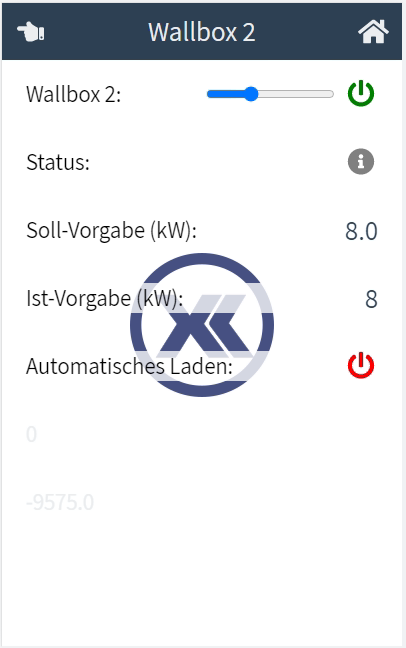
\includegraphics[scale=0.5]{pics/DetailansichtWallbox2.png}
  \caption{Detailansicht der Oberfläche für die Einzelnen Wallboxen }
  \label{fig:impl:HMIWallboxDetail}
\end{figure}

Siehe Deteilansicht der Wallbox: \ref{fig:impl:HMIWallboxDetail}.

